\section{Introduction}

\subsubsection{Historical context}

%Summarize the scientific question that your code was written to explore.
This paper aims to computationally reproduce my own statistical analysis from 16~years ago as part of the 10-year reproducibility challenge \supercite{Hinsen2019}. The analysis examined seasonal patterns in cardiovascular disease in multiple countries \supercite{Barnett2004}. In most countries cardiovascular deaths and emergency admissions to hospital have a strong seasonal pattern with a peak in winter and nadir in summer \supercite{Stewart2017}. There is an interesting variability between-countries in the size and timing of the winter peak. A better understanding of the differences between countries could help our understanding of the underlying causes of the winter peak in disease.

The analysis examined monthly time series of cardiovascular events (fatal and non-fatal) from 35~locations in 21~countries. The time series were 8 to 14 years in length and the earliest year of data was 1980. The analysis aimed to split the time series into a long-term trend, seasonal patterns and residual. There were two approaches, one that used a two-stage approach by first removing the trend, and another that estimated the trend and season together. The trend was estimated using the Kalman filter and the seasonal patterns were estimated using sinusoids. The estimates were made using Markov chain Monte Carlo. 

%Describe the computational context: Which hardware was used to run the code? Which software infrastructure? Which constraints existed on software development? Which technical choices (language, libraries, ...) were made? Were reproducibility and/or re-usability important criteria?

\subsubsection{Original source code}

The original code was written in SAS (version~8.00 for Windows) and chain convergence was checked using the ``coda'' package (version unknown) in R \supercite{coda}. The code was based on Matlab code that I wrote during my PhD \supercite{Barnett2003}. I converted the code to SAS because I did not have access to Matlab after finishing my PhD and I hoped that more people would be able to re-use my SAS code to apply to their own data. It was not common practice at the time to share code and data in order to allow others to reproduce results. The SAS code was first published in November 2004 with an update in August 2006, but there is no record of what changes were made. 

%About the original source code: Was it published? Was it archived somewhere? Was there a license for it?
The original code was published in an online appendix to the paper that was separate from the journal in November 2004 at this address: \url{http://www4.ktl.fi/publications/monica/chd_seasonal/appendix.htm}. However, the site has since moved to: \url{https://www.thl.fi/publications/monica/chd_seasonal/appendix.htm} (accessed 25 January 2020). The web site was created by the WHO MONICA Project specifically for appendices to papers that used the MONICA data. MONICA stands for monitoring trends and determinants in cardiovascular disease. The MONICA Project was a large multi-country study that aimed to examine several aspects of cardiovascular disease \supercite{Tunstall2003}. It was a well-managed project that had staff who assisted with access to the data and helped add my code to the web.  

The paper states the code was published in September 2002 but this is likely a mistake given that the paper was not submitted until January 2004. 

%Please provide only information you are certain about. It's OK to forget technical details after many years.

\section{Results}

%Retrieval of the software
%Was it easy to find a copy of your source code?
%Was it easy to locate and setup the dependencies?
%Provide a list of all dependencies (libraries but also tools such as compilers).

\subsubsection{Retrieval of the software}

Most of my SAS code was easy to find, both on the web and on an old CD in a desk draw. I made this CD of my files when I moved jobs. I did not keep the data because I was more interested in other people using my code for their own data rather than replicating our published results. I believe that another reason for deleting the data was to save space, as the files were relatively large by the standards of the day (around 31,000~kilobytes for data in text format and 70,000~kilobytes for data in SAS format). Luckily the original data files were available in a CD attached to the MONICA monograph published in 2003 \supercite{Tunstall2003}.

My SAS code contained the macros needed to run the two statistical analyses. There was also SAS code to simulate a seasonal time series as an example data set. I found SAS code to read the MONICA data on my CD, but not on the web. I could not find the SAS code that applied the two methods to each location.

%Execution
%Describe what you did in order to run the software today.
%Did you succeed in running the software in a modern computational environment? Or did you have to search for old versions of tools and libraries?
%Describe the computational environment of the reproduction: hardware, operating system, compiler versions etc.
%Did you have to modify the software in order to make it run today?
%Were the original instructions that came with the software sufficient, or did you have to modify or extend them?

\subsubsection{Replication execution}

I used SAS version~9.4 for Windows (Microsoft Windows~10) to replicate the results; there was no need to use an earlier version of SAS. 

My SAS files had relatively good instructions with a detailed header at the top of every file and comments throughout. However, some files had been adapted from the original analysis to secondary analyses, making the code a palimpsest with some commands commented out with notes such as, ``changed for weather analysis'' and ``sensitivity analysis of Ghent''. The correct data set was also ambiguous because alternative data sets had also been used (e.g., fatal vs non-fatal events).  In hindsight I should have kept the exact data and syntax files needed to re-create the published results.
%Mix of SAS files from different projects in the same folder.

The macros to run the analyses mainly needed only cosmetic edits, and I also put each macro in its own file rather than one overall file of macros. I also moved part of one macro, that estimated the standard deviation of the noise, into the macro that tested the periodogram for remaining seasonal structure. The largest change was having to re-write the files that applied the macros to the MONICA data. My SAS programming was rusty and I could not automate the process for each centre, so instead I created a new file for each analysis in each of three centres.

I did not repeat my analysis in all 35 locations, but instead did the three in the first figure as this felt sufficient to test the code.

The code to estimate the trend without the seasonal pattern used a slightly different parameterisation with ``tau'' as a ratio rather than an absolute value. ``tau'' controls the amount of change over time in the trend, with smaller values creating more linear trends. I cannot be sure that this version was the same code as the original, although it produced similar results.

%One small modification was to change the library locations.

%\clearpage
\subsubsection{Closeness of the replicated results to the original}

%How close were the results you got to the originally published ones? Include the replicated data table and figure, as we do in other ReScience articles.
The original figure is replicated in Figure~\ref{fig}, which shows the estimates of the trend and season for three locations.
The results are very similar bar one issue: the confidence intervals for the trend, which are much narrower for the replication, but are centred on a similar mean.
This may be because I could not be certain that I had found the original code to perform the Kalman filter smoothing because of the difference in how ``tau'' was parameterised. However, the estimates do look remarkably similar to my replicated estimates of the trend using the combined method. Hence it is possible that the original figures were mislabeled as being from the two-stage method when in fact they came from the combined method.

\begin{figure}[!h]
\centerline{Perth, Australia}
	\centerline{
    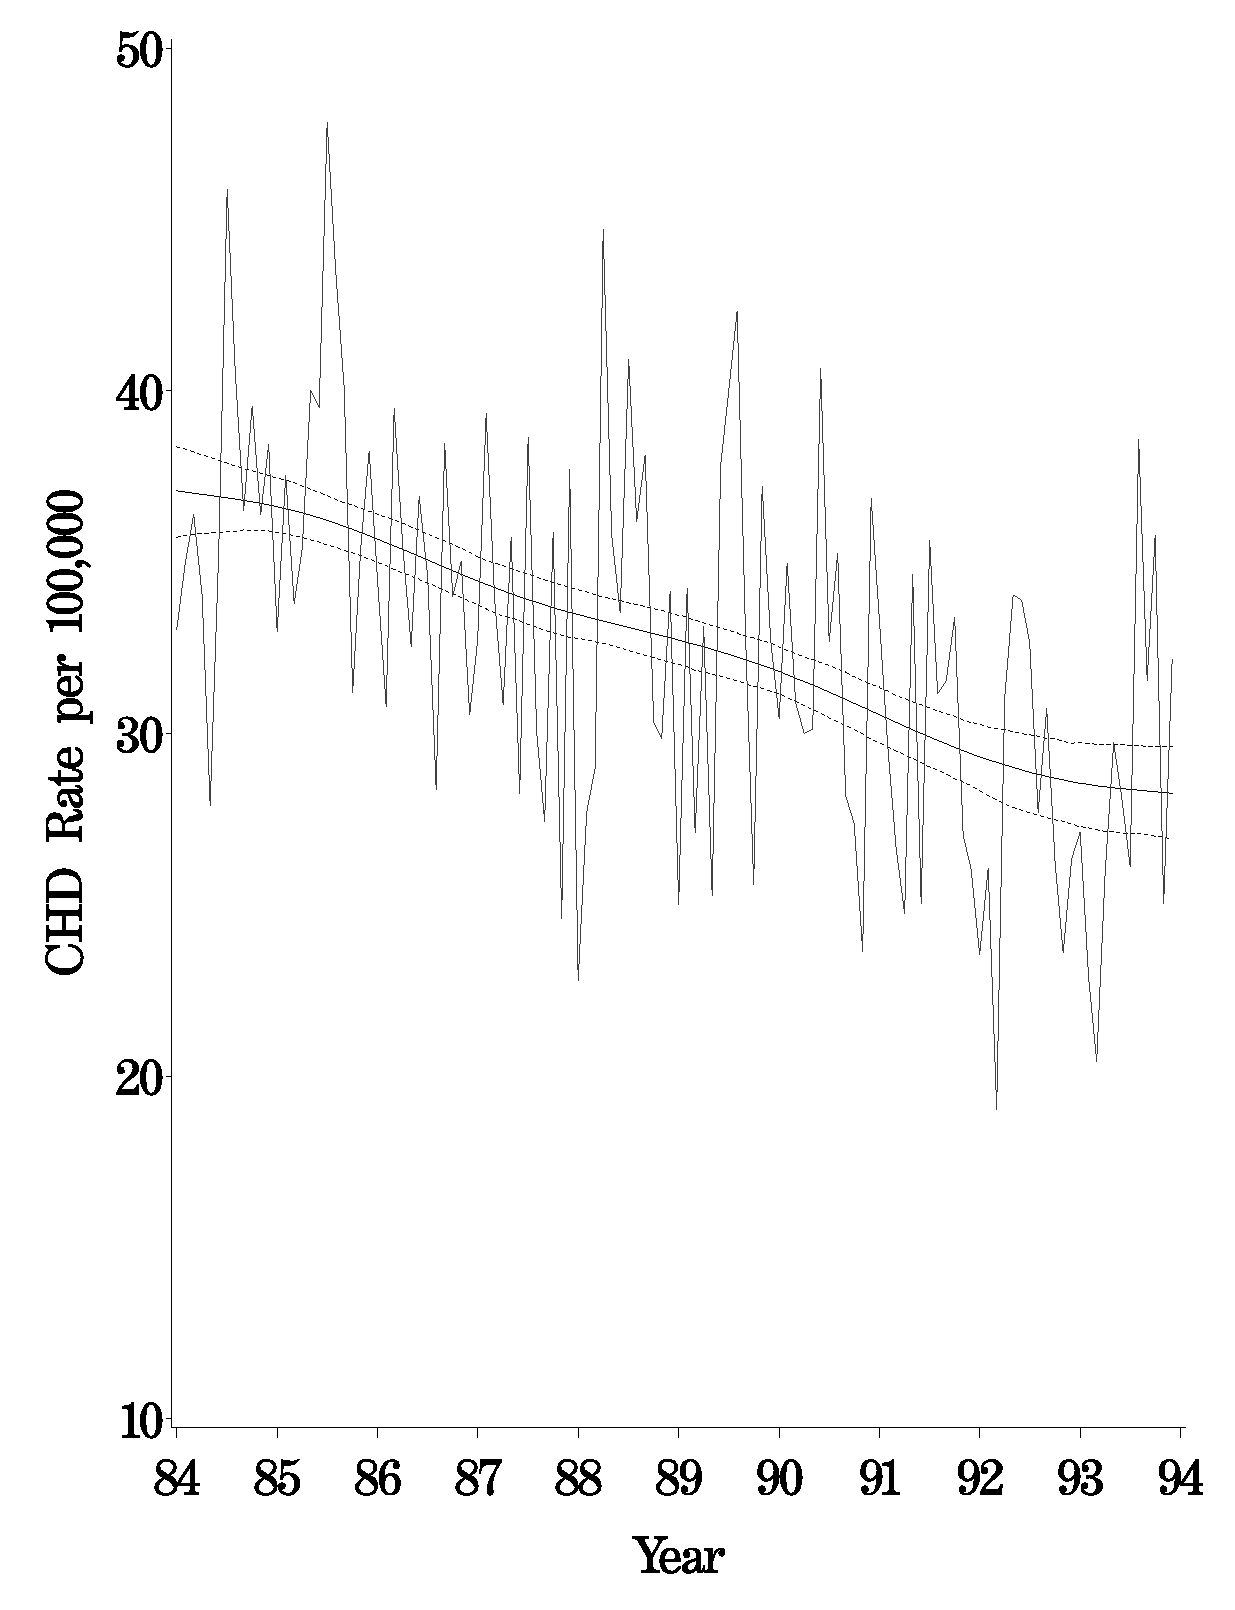
\includegraphics[scale=0.2]{figures/trend_twostage_perth.eps}
    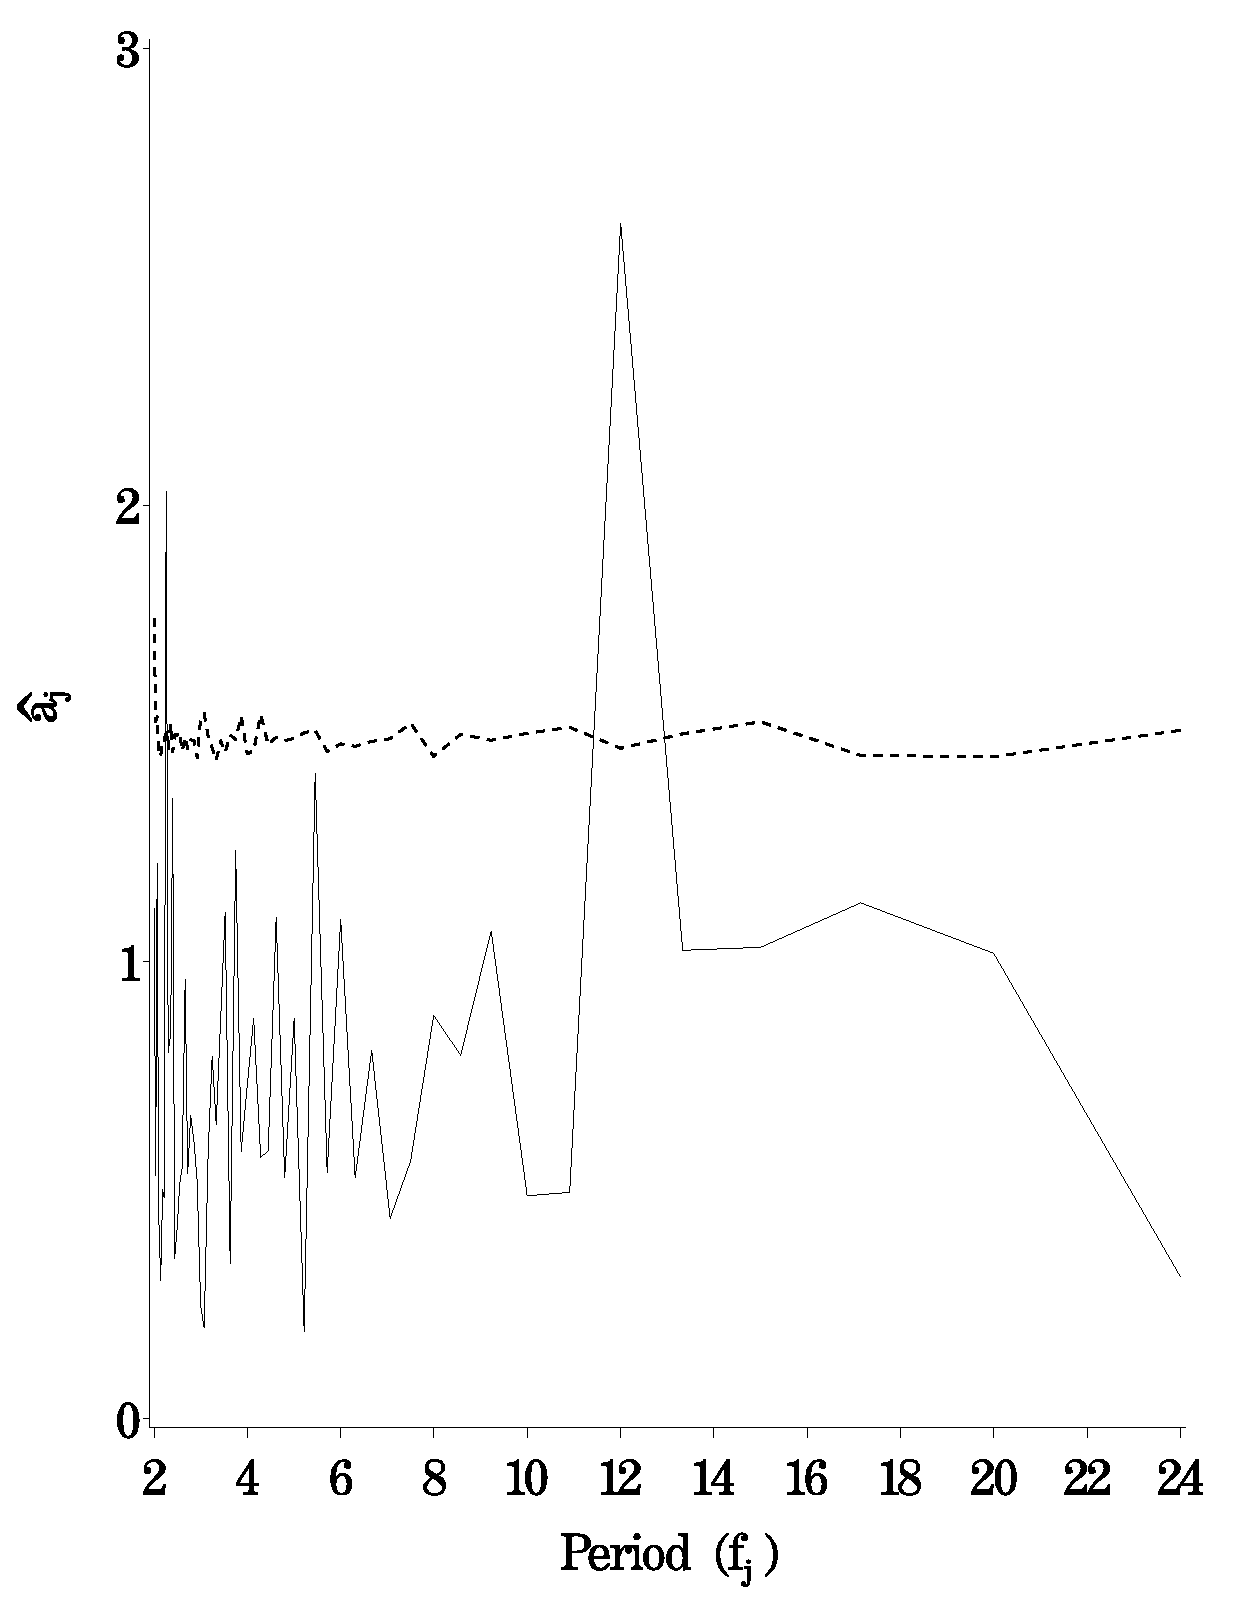
\includegraphics[scale=0.2]{figures/periodogram_twostage_perth.eps}
    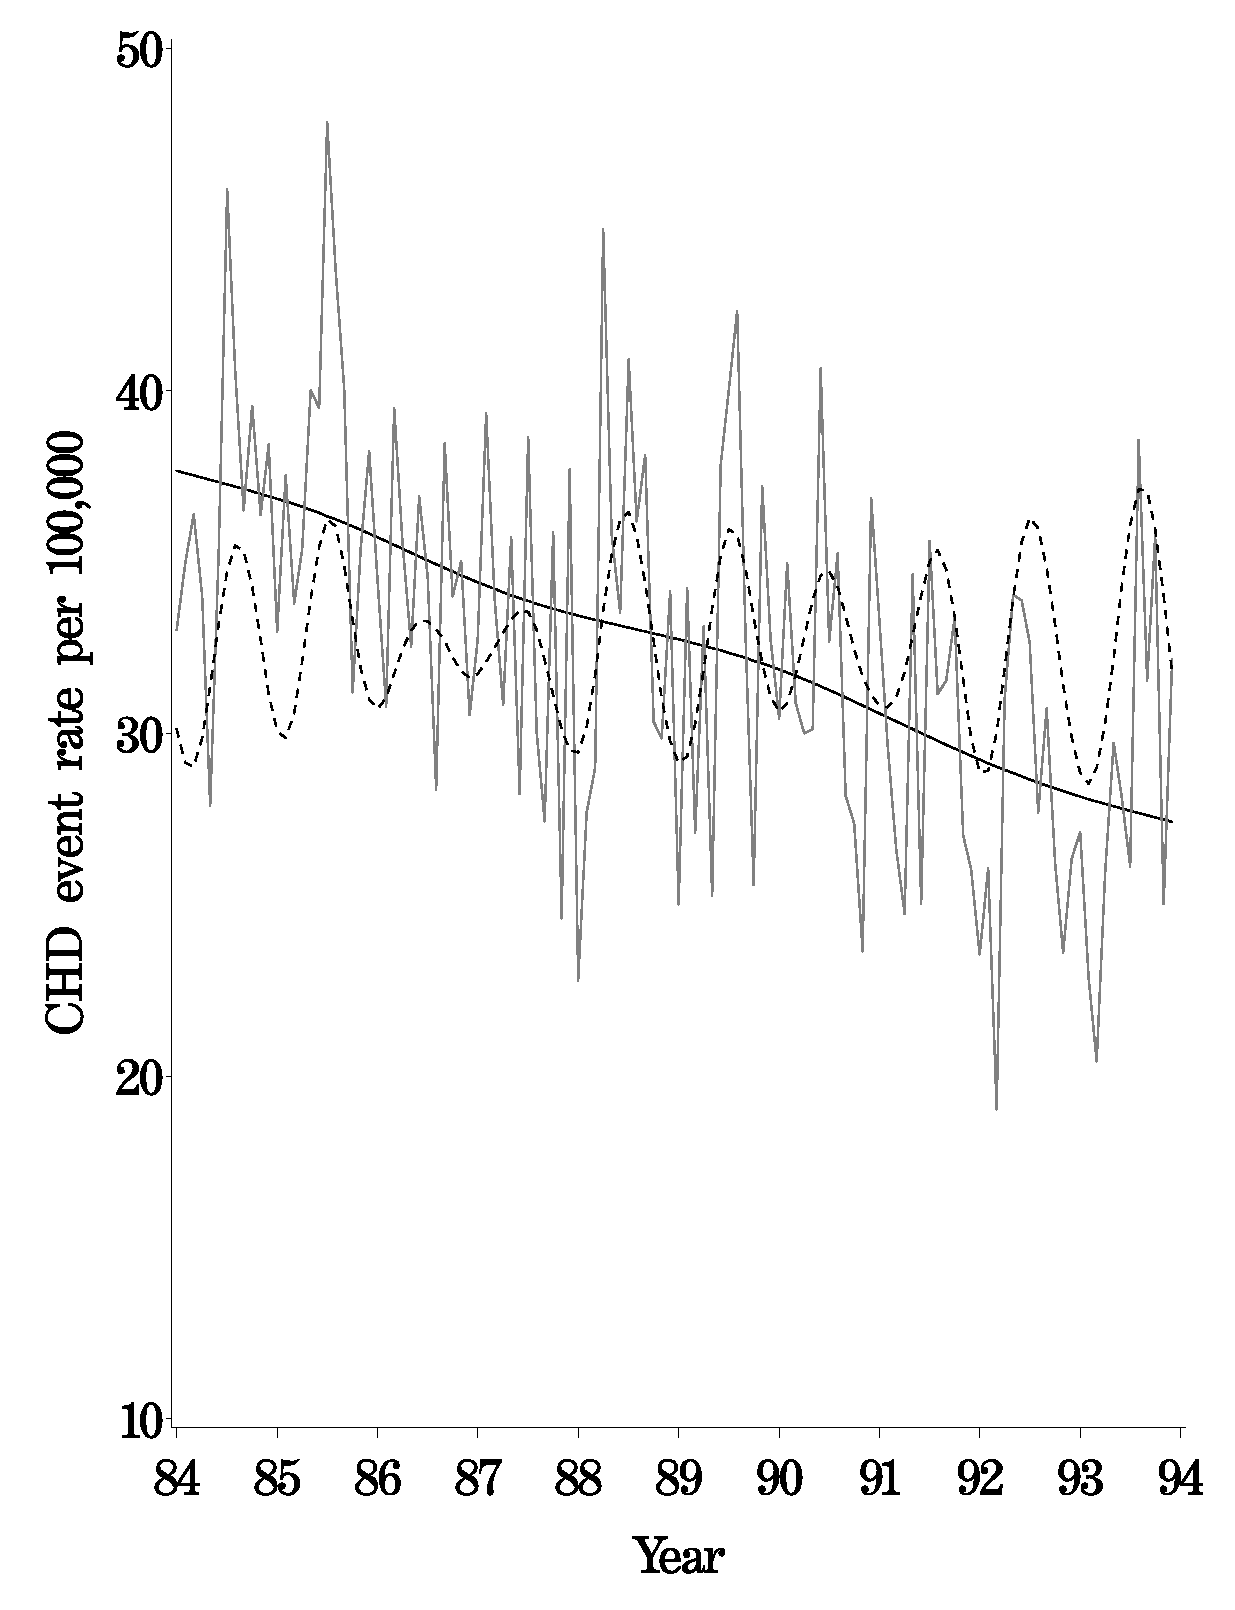
\includegraphics[scale=0.2]{figures/estimates_combined_perth.eps}
    }

\centerline{Belfast, UK}
    \centerline{
    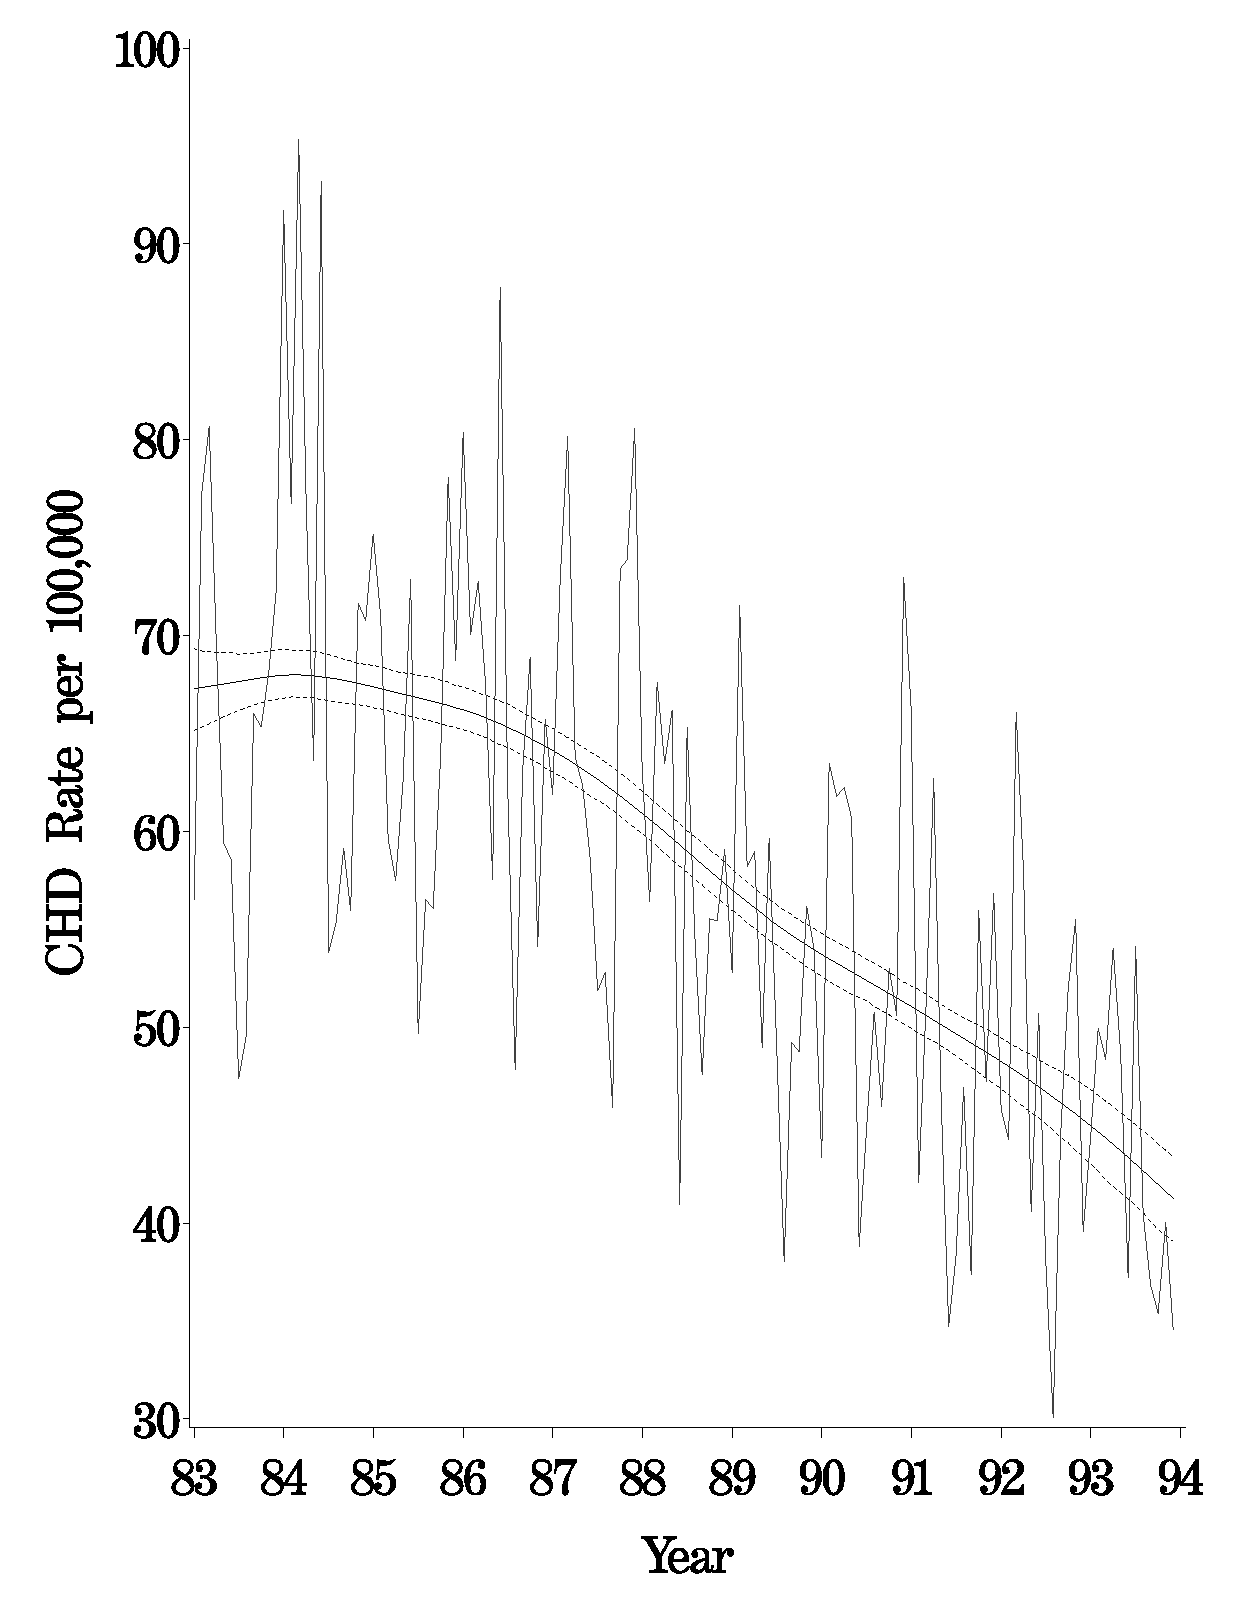
\includegraphics[scale=0.2]{figures/trend_twostage_belfast.eps}
    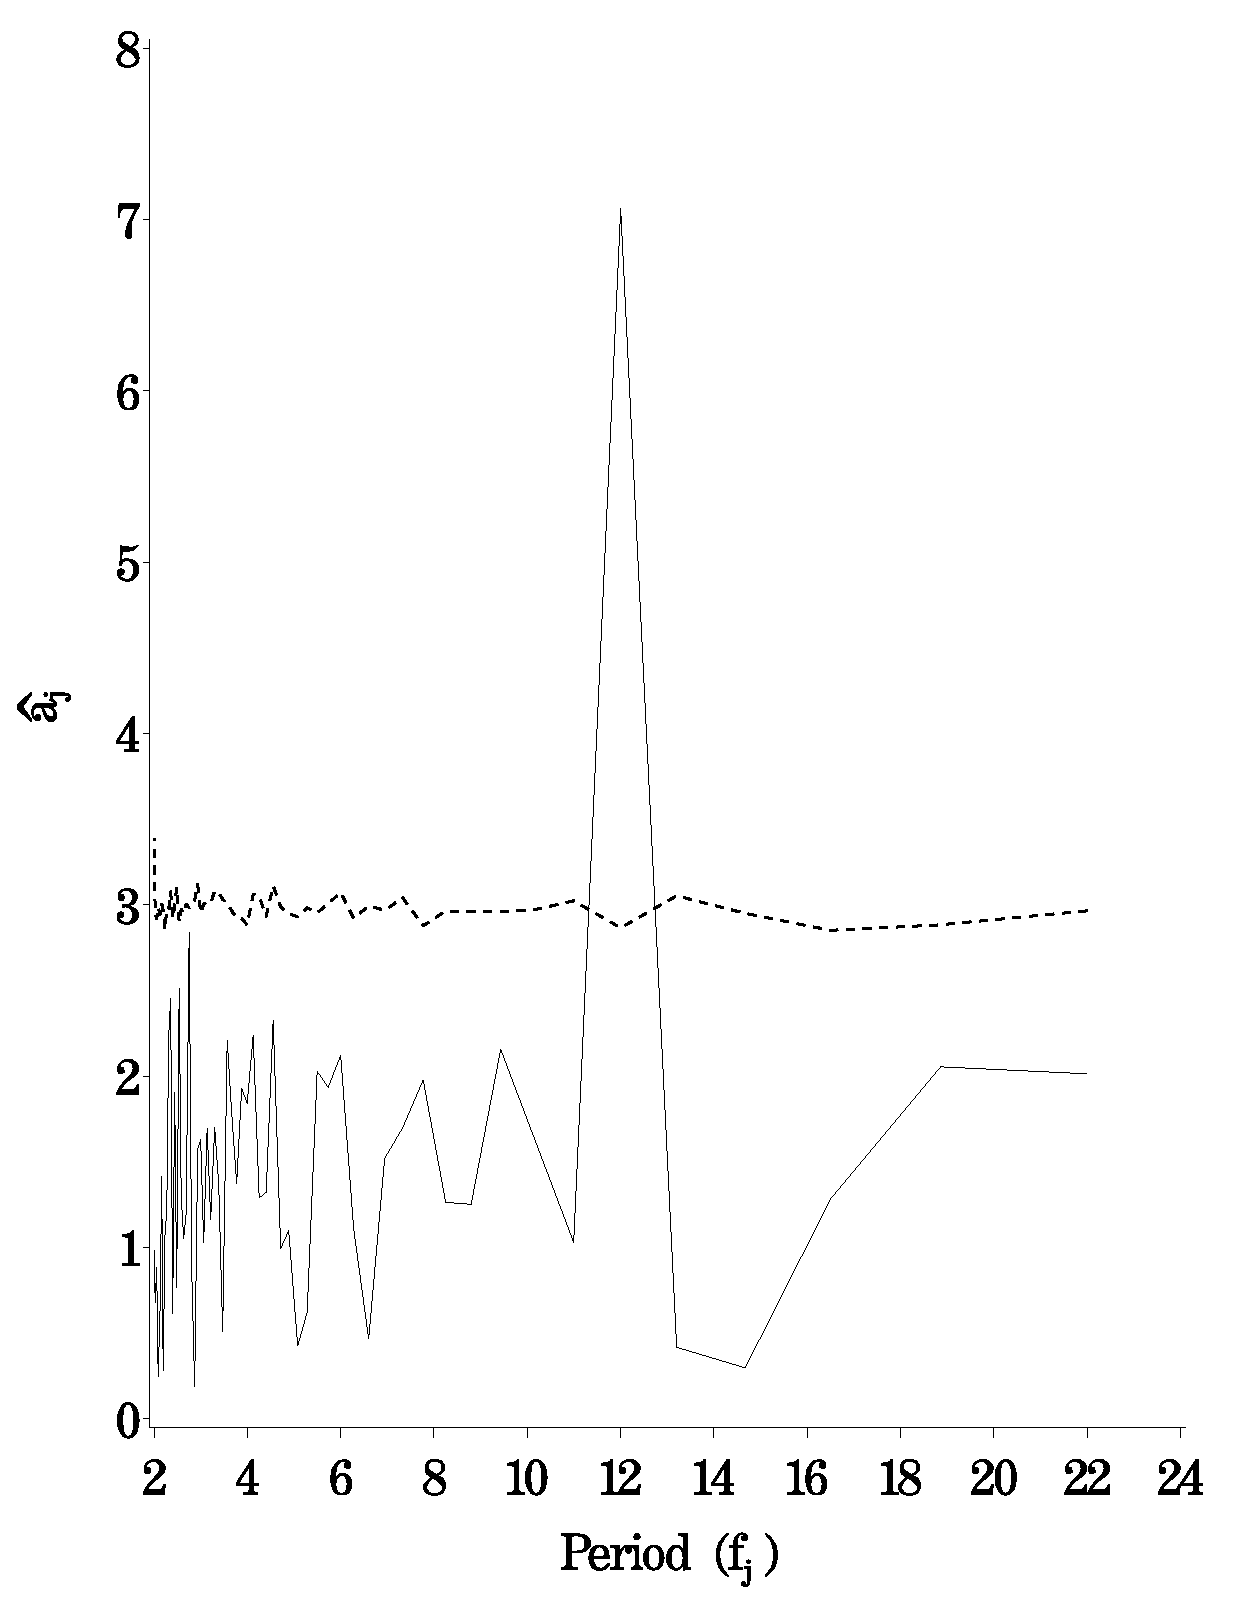
\includegraphics[scale=0.2]{figures/periodogram_twostage_belfast.eps}
    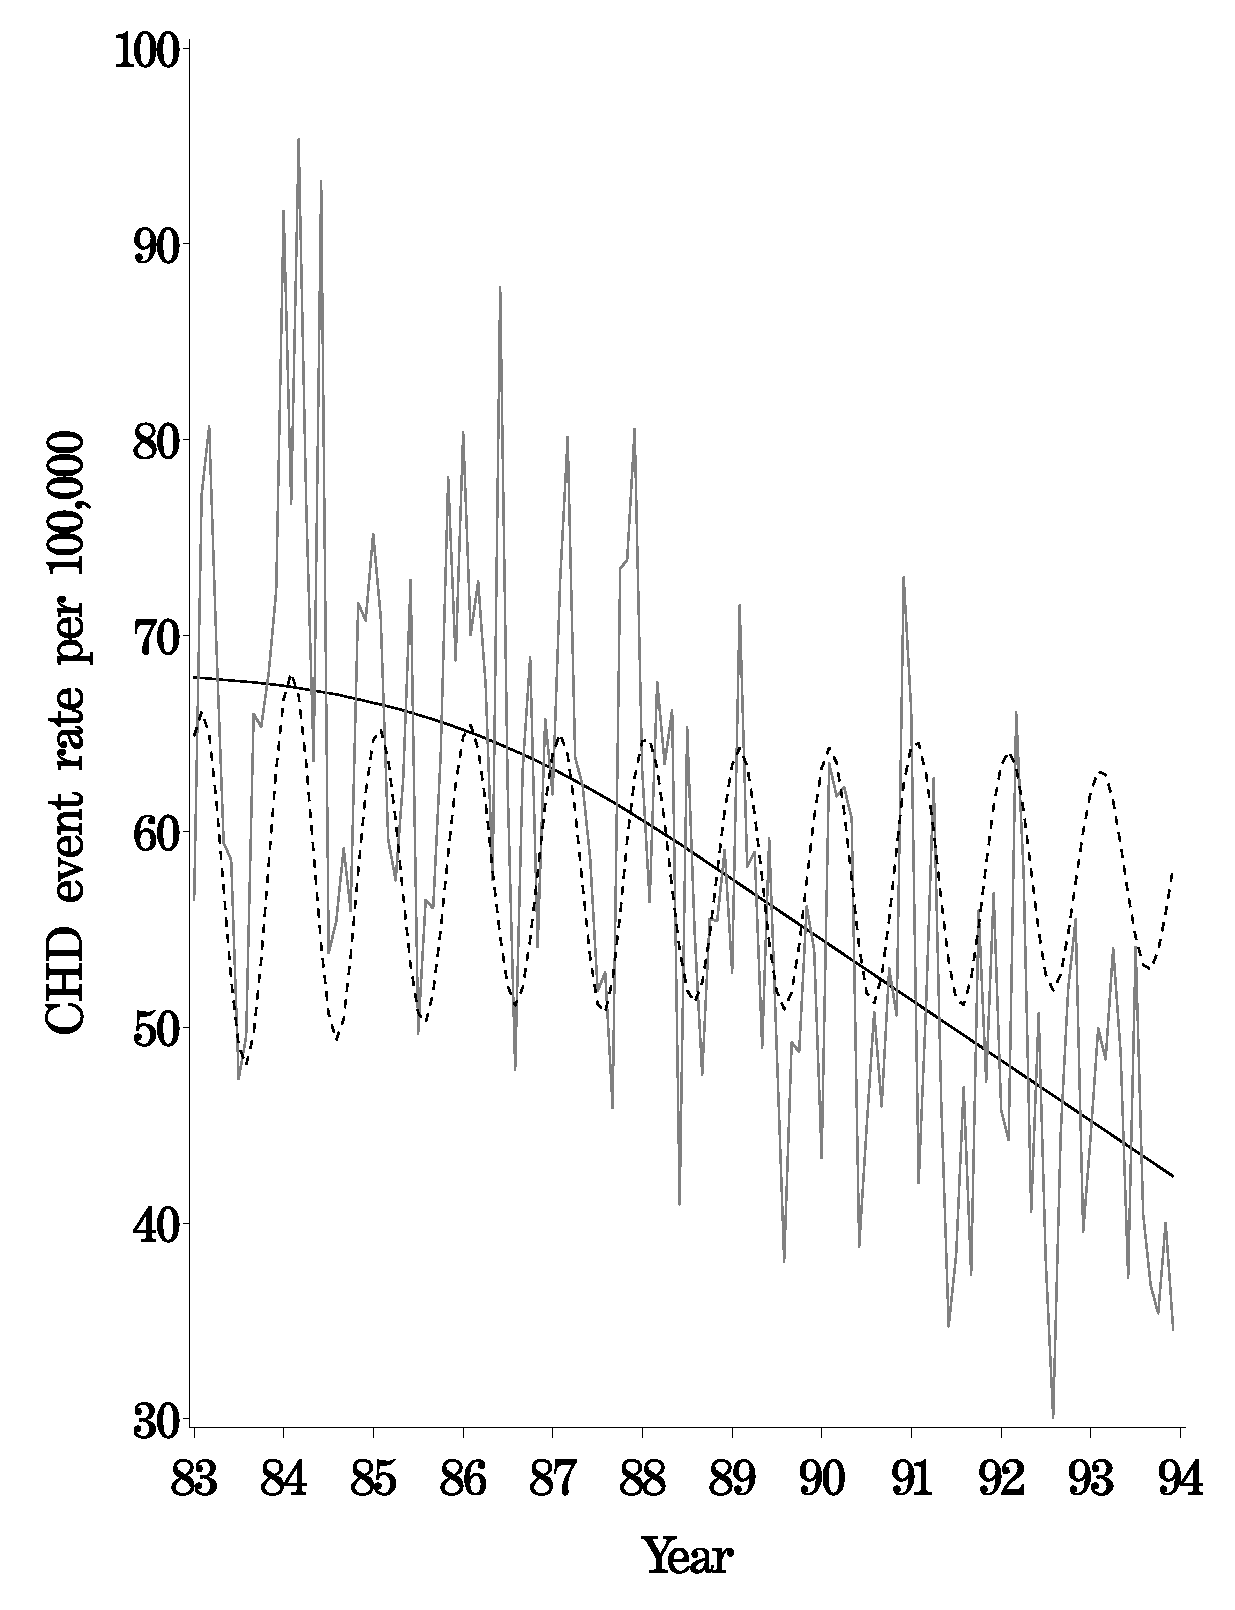
\includegraphics[scale=0.2]{figures/estimates_combined_belfast.eps}
    }

\centerline{Warsaw, Poland}
    \centerline{
    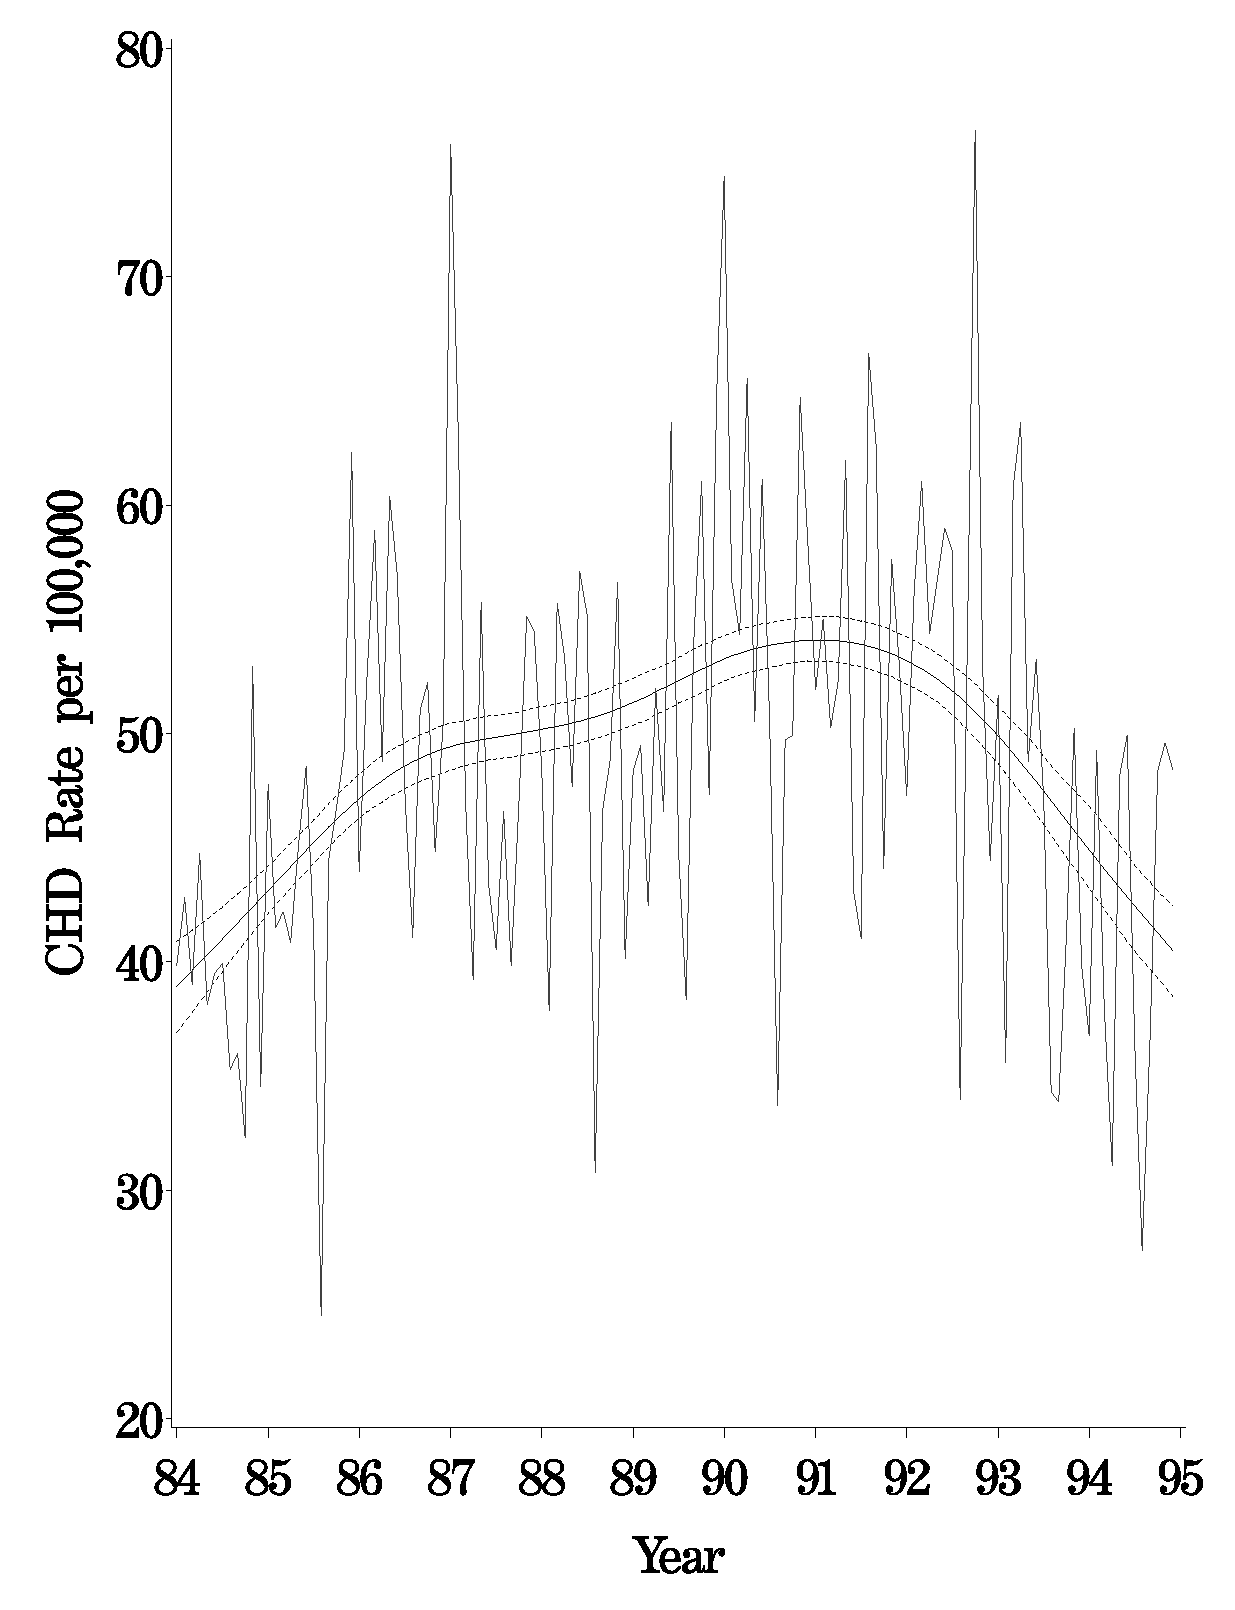
\includegraphics[scale=0.2]{figures/trend_twostage_warsaw.eps}
    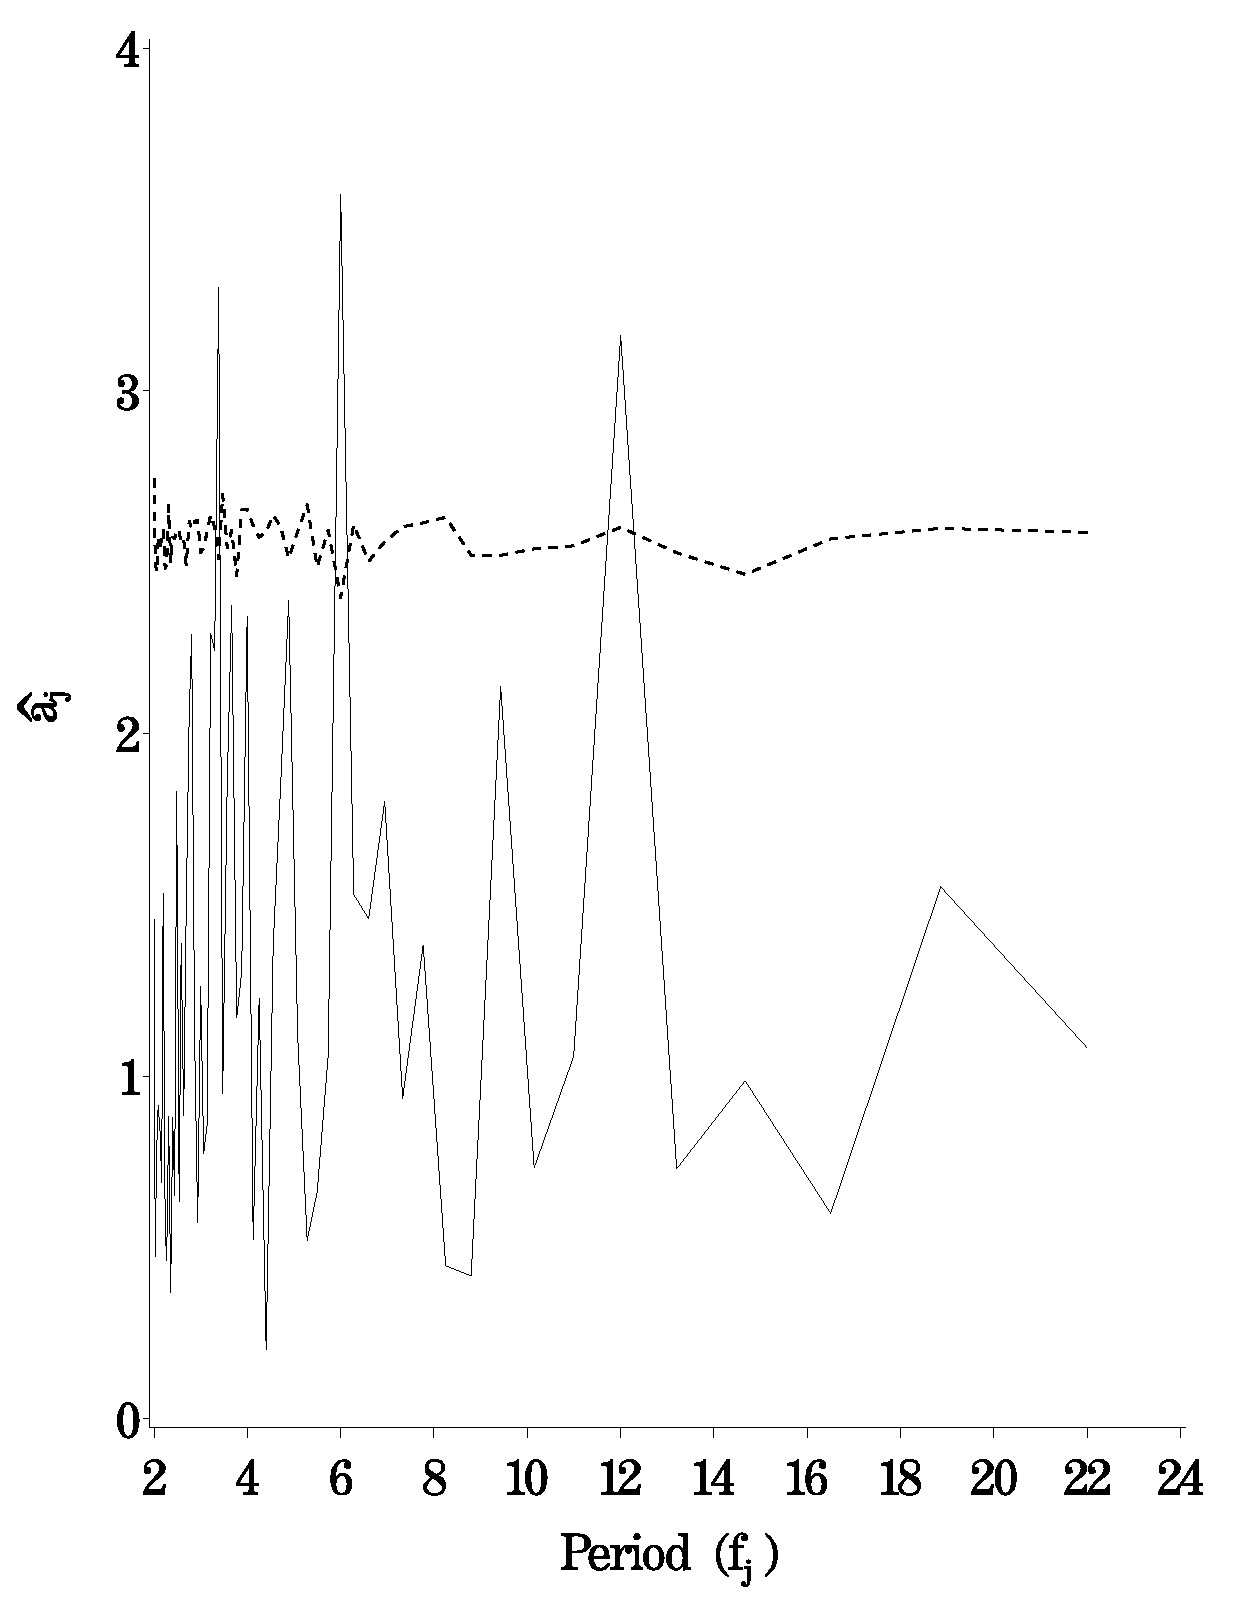
\includegraphics[scale=0.2]{figures/periodogram_twostage_warsaw.eps}
    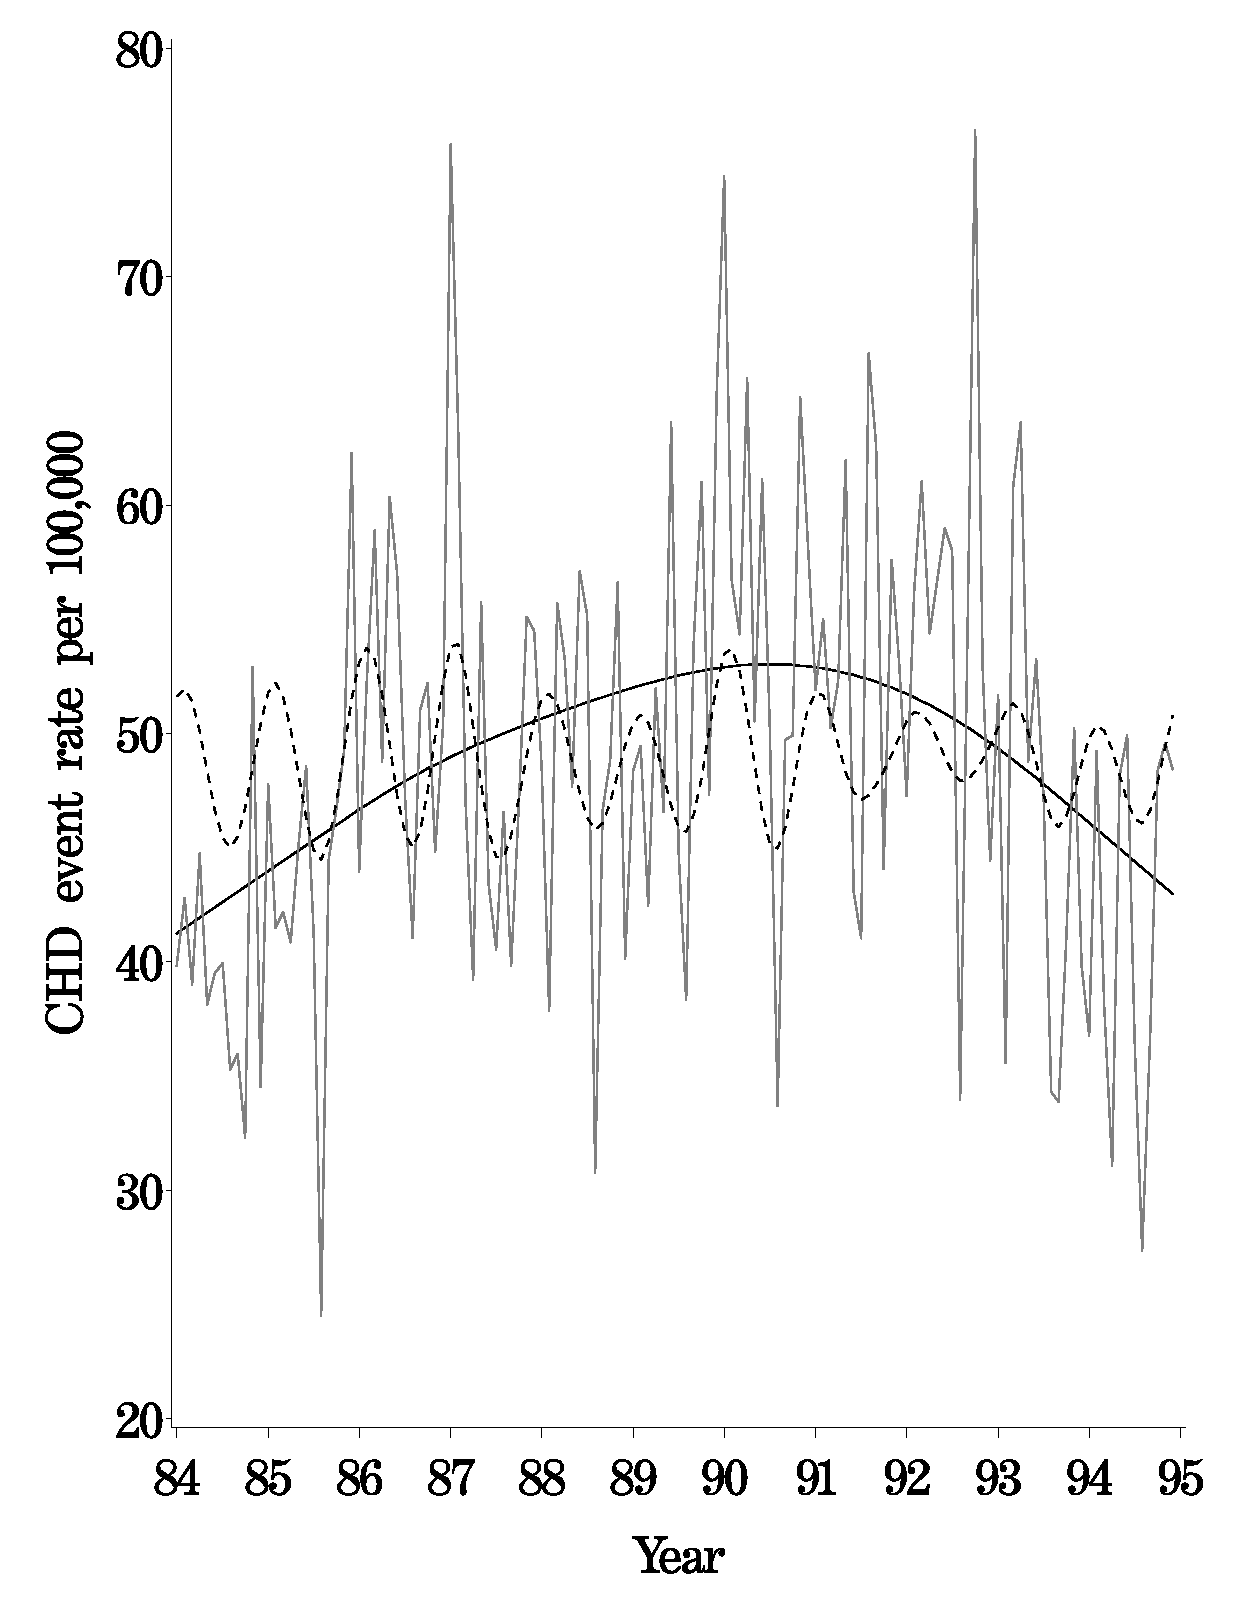
\includegraphics[scale=0.2]{figures/estimates_combined_warsaw.eps}
    }

\caption{Replicated results for three locations using the two-stage method (left and centre column) and combined method (right column). The left column shows the observed data, estimated trend and 95\% confidence interval. The middle column shows the periodogram of the de-trended data and limit for the test of seasonal structure (dotted line). The right column shows the observed data, estimated trend, and estimated annual seasonal pattern.}
	\label{fig}
\end{figure}

The seasonal estimates for the three locations in Figure~\ref{fig} are replicated in Table~\ref{tab:season} which also shows the original results. The results are similar for the two-stage method, with the biggest difference being for the estimate of the noise standard deviation (4.8 versus 4.2).
The results are presented
How similar?

\begin{table}[!h]
  \centering
  \begin{tabular}{rccc}\hline
 & Frequency,  & Amplitude,  &  Noise \\ 
Location & months & rate per 100,000 &  SD \\ \hline
\multicolumn{4}{c}{Two-stage} \\ \hline
Perth, Australia & 2.3 & 2.0 (2.0) & 4.8 (4.2)\\
 & 12 & 2.6 (2.6) \\
Belfast, UK & 12 & 7.1 (7.0) & 8.7 (8.7) \\ 
Warsaw, Poland & 3.4 & 3.3 (3.3) & 7.5 (7.5)\\
               & 6  & 3.6 (3.6)\\ 
               & 12 & 3.2 (3.2)\\
\hline
\multicolumn{4}{c}{Combined}  \\ \hline
Perth, Australia & 2.3 & 1.0 (1.0) & 3.9 (3.9)\\
 & 2.7 & ---- (0.8) \\
 & 3.8 & 1.3 (1.3)\\
 & 5.5 & 1.5 (1.4)\\
 & 12 & 2.7 (2.7)\\
Belfast, UK & 2.8 & ---- (1.6) & 9.0 (8.8) \\
            & 12 & 7.1 (7.0) &  \\ 
Warsaw, Poland & 3.4 & 3.4 (3.4) & 7.9 (7.8)\\
               & 6  & 3.7 (3.7)\\ 
               & 12 & 3.3 (3.3)\\
\hline
\end{tabular}
 \caption{Estimates of seasonal patterns using the two-stage and combined methods for three locations. The original results are in brackets. Each row in the table corresponds to a seasonal frequency at a location. SD = standard deviation.}
  \label{tab:season}  
\end{table}

There were differences in the frequencies for the combined method, as two seasonal frequencies were not included in the new results, one in Perth and one in Belfast. Although the amplitudes were relatively small (1.6 or less), hence these are smaller seasonal patterns.

This difference could be because of a key ambiguity in the original paper regarding the decision to add additional seasonal components for the combined approach. After fitting a model the residuals were tested to look for additional seasonal structure. If structure existed, then the model was modified to add an additional seasonal component as necessary, followed by another test of the residuals. The code produced both the periodogram and the spectrum, which is a smoothed version of the periodogram. The periodogram tended to flag significant seasonal patterns when the spectrum did not, and I used the spectrum to make the decisions because some of the statistically significant patterns found by the periodogram were only just above the 0.05 threshold used to judge statistical significance. This part of the replication was therefore somewhat subjective.

Some of the discrepancy in results could be because the estimates are made using Markov chain Monte Carlo which uses random steps to make estimates. Hence the estimates will depend on the original random number seed. However, I used 5,000 estimates with a burn-in of 500, so these differences should be minor and may explain some of the small differences in the first decimal place for the amplitude and noise estimates.

%If you had to make any modifications to the software or to the instructions that were supplied with it, try to describe which competence another researcher would need in order to do the same work. Would a general familiarity with your programming language and environment have been sufficient?

Overall the replication took about 20~hours. This was mostly the fiddly task of working out which macros to run and re-creating the figures and tables. Given the amount of code that had to be re-created, I think that only someone very familiar with SAS would have been able to replicate the results. My familiarity with the MONICA Project also helped me create the new code, hence I am not certain that an outsider could have replicated the results, perhaps only by trial-and-error.

%Software
%If the licenses applying to the original software allow, please make your old software available as a repository on GitHub or an equivalent site. In the best case scenario, in which the old code is publishable, here is the procedure:

%Add your old software as a single commit (ideally the initial one) of a new source repository.
%Edit the code as necessary to reproduce the results in today's computational environment, committing the changes in logical units in the process. Include the additional tools (scripts, makefiles, ...) that you wrote for re-running your software and the additional instructions.
%Make sure your repository contains a license.
%Finally, submit your repository to Software Heritage for archiving.

\section{Discussion}

%In addition to the content covered below, we are interested in the insight resulting from the reproducibility experience in relation to the choice of technology, and in your opinion on the original source code (clarity, documentation, etc).

It was an interesting exercise to bring this old code back to life. It would have been easier and faster if my original code had been properly arranged and prepared solely to repeat the original analyses. However, I was not aware of guidelines for curating code back in 2004. My original code had many comments which were useful, but there were problems with the overall file structure and how the files related to one another. There were also ambiguities with the dates of the code, and the changes I made after posting the original files. This is now solved by sites that track and date-stamp all changes, such as \textit{GitHub}.

My main reason for sharing the original code was so that others could adapt it to their own data. However, of the 21 papers that cited the original paper which I could access, none of them stated that they re-used my SAS code. 
%I was not focused on the nitty-gritty of reproducing the original results and my code was in bad shape to do this.

% One instead cited the available R code to run the same analysis.
% Not confident it was exactly the same, but broadly similar.

Overall the replication was broadly successful in terms of re-creating the key figure and estimates for three locations. There was some subjectivity in modelling decisions, which made perfect replication hard.

%The ``combined'' model in the SAS files are available in the ``season'' package in R \supercite{season} using the ``nscosinor`` command.